\documentclass{exam}
\usepackage{graphicx} 

% Format Header and footer
\pagestyle{headandfoot}
\header{\footnotesize Klass:\\Namn:}{\Large\textbf{Fysiologi II}\\\medskip\small Nervsystemet, rörelseapparaten och endokrina organsystemet}{\footnotesize BIOBIO02 - 2025\\Viktor Arohlén}
\headrule
\footrule
\setlength{\columnsep}{0.25cm}
\footer{}{Sida \thepage}{}

\begin{document}
\section*{Instruktioner}
Provet består av två delar \\
    - Grundläggande frågor, svara kortfattat (\textit{14 poäng})\\
    - Fördjupande frågor, svara mer omfattande (\textit{10 poäng} + 2 bonuspoäng)

\subsection*{Poäng}
Antalet poäng är markerat för varje fråga. Totalt \textbf{12 frågor} och \textbf{24 poäng}.\\ \textit{För godkänt resultat krävs 10 poäng.}

\vspace{5mm} %5mm vertical space
\begin{center}
\fbox{\fbox{\parbox{6in}{\centering
\textbf{Grundläggande frågor}: svara kortfattat (\textbf{14 poäng})
}}}
\end{center}
\begin{questions}

\question I vilken ordning sker signalöverföringen i en synaps? (\textbf{2 poäng})

\begin{itemize}
  \item Aktionspotential når axonterminalen
  \item Neurotransmittorer frisätts
  \item Jonkanaler öppnas i postsynaptiska membranet
  \item Spänningsförändring i postsynaptiska cellen
  \item Vesiklar med neurotransmittorer fuserar med cellmembranet
  \item Neurotransmittorer binder till receptorer
\end{itemize}

\vspace{5mm} %5mm vertical space

\question Beskriv två olika typer av \textbf{leder} i människokroppen och ge exempel på var de finns. (\textbf{2 poäng})
\vspace{40mm}

\question Vad av följande är \textbf{inte} ett hormon? (\textbf{1 poäng})
\begin{checkboxes}
    \choice Insulin
    \choice Acetylkolin
    \choice Kortisol
    \choice Tyroxin
\end{checkboxes}

\vspace{5mm}
\question Vad av följande \textbf{stämmer} om nervsystemet? (\textbf{1 poäng})
\begin{checkboxes}
    \choice Parasympatiska nervsystemet aktiveras vid fysisk ansträngning
    \choice Sympatiska nervsystemet sänker hjärtfrekvensen
    \choice Somatiska nervsystemet styr viljestyrda rörelser
    \choice Autonoma nervsystemet kontrollerar skelettmuskulatur
\end{checkboxes}
\break

\question Beskriv skillnaden mellan de olika typerna av \textbf{muskelvävnad} och deras funktion. (\textbf{2 poäng})
\vspace{40mm}

\question Vad av följande \textbf{stämmer} om det endokrina systemet? (\textbf{1 poäng})
\begin{checkboxes}
    \choice Hypofysen kontrolleras av njurarna
    \choice Sköldkörteln producerar insulin
    \choice Binjurarna producerar stresshormoner
    \choice Bukspottkörteln reglerar kalciumbalansen
\end{checkboxes}

\vspace{5mm}
\question Beskriv \textbf{tre} viktiga funktioner som skelettet har i kroppen. (\textbf{2 poäng})
\vspace{40mm}

\question Vad av följande \textbf{stämmer} om hjärnan? (\textbf{1 poäng})
\begin{checkboxes}
    \choice Lillhjärnan ansvarar för medveten tankeverksamhet
    \choice Hjärnstammen kontrollerar känslor
    \choice Storhjärnan är uppdelad i fyra lober
    \choice Hypotalamus är en del av det limbiska systemet
\end{checkboxes}
\vspace{5mm}

\question Vilket av följande påståenden om neurotransmittorer är korrekt? (\textbf{1 poäng})
\begin{checkboxes}
    \choice Neurotransmittorer frisätts från nervcellens axonterminal och binder till receptorer på mottagarcellens membran.
    \choice Alla neurotransmittorer verkar genom att hämma nervimpulser.
    \choice Dopamin är en neurotransmittor som endast finns i muskler.
    \choice Serotonin påverkar stämningsläget.
\end{checkboxes}


\break

\vspace{5mm} %5mm vertical space
\begin{center}
\fbox{\fbox{\parbox{6in}{\centering
\textbf{Fördjupande frågor}: svara mer utförligt (\textbf{10 poäng} + 2 bonuspoäng)
}}}
\end{center}

\question
Förklara vad Viktor menar när han säger att hjärnstammen är den "evolutionärt äldsta" och storhjärnan den "evolutionärt yngsta" delen av CNS? (\textbf{2 poäng})
\vspace{60mm}

\question
Förklara hur nervsystemet och det endokrina systemet samverkar för att upprätthålla homeostas. Ge ett konkret exempel på denna samverkan. (\textbf{2 poäng})

\vspace{60mm}
\question
Beskriv skillnaderna mellan \textbf{endoskolett, exoskelett och hydrostatiskt skelett}. Vad är för och nackdelarna med de olika typerna? (\textbf{2 poäng})
\vspace{60mm}

\break

\question Nedan ses en bild av en nervcell. Med bilden som hjälp besvara följande frågor: (\textbf{4 poäng})
\begin{figure}[h]
\centering
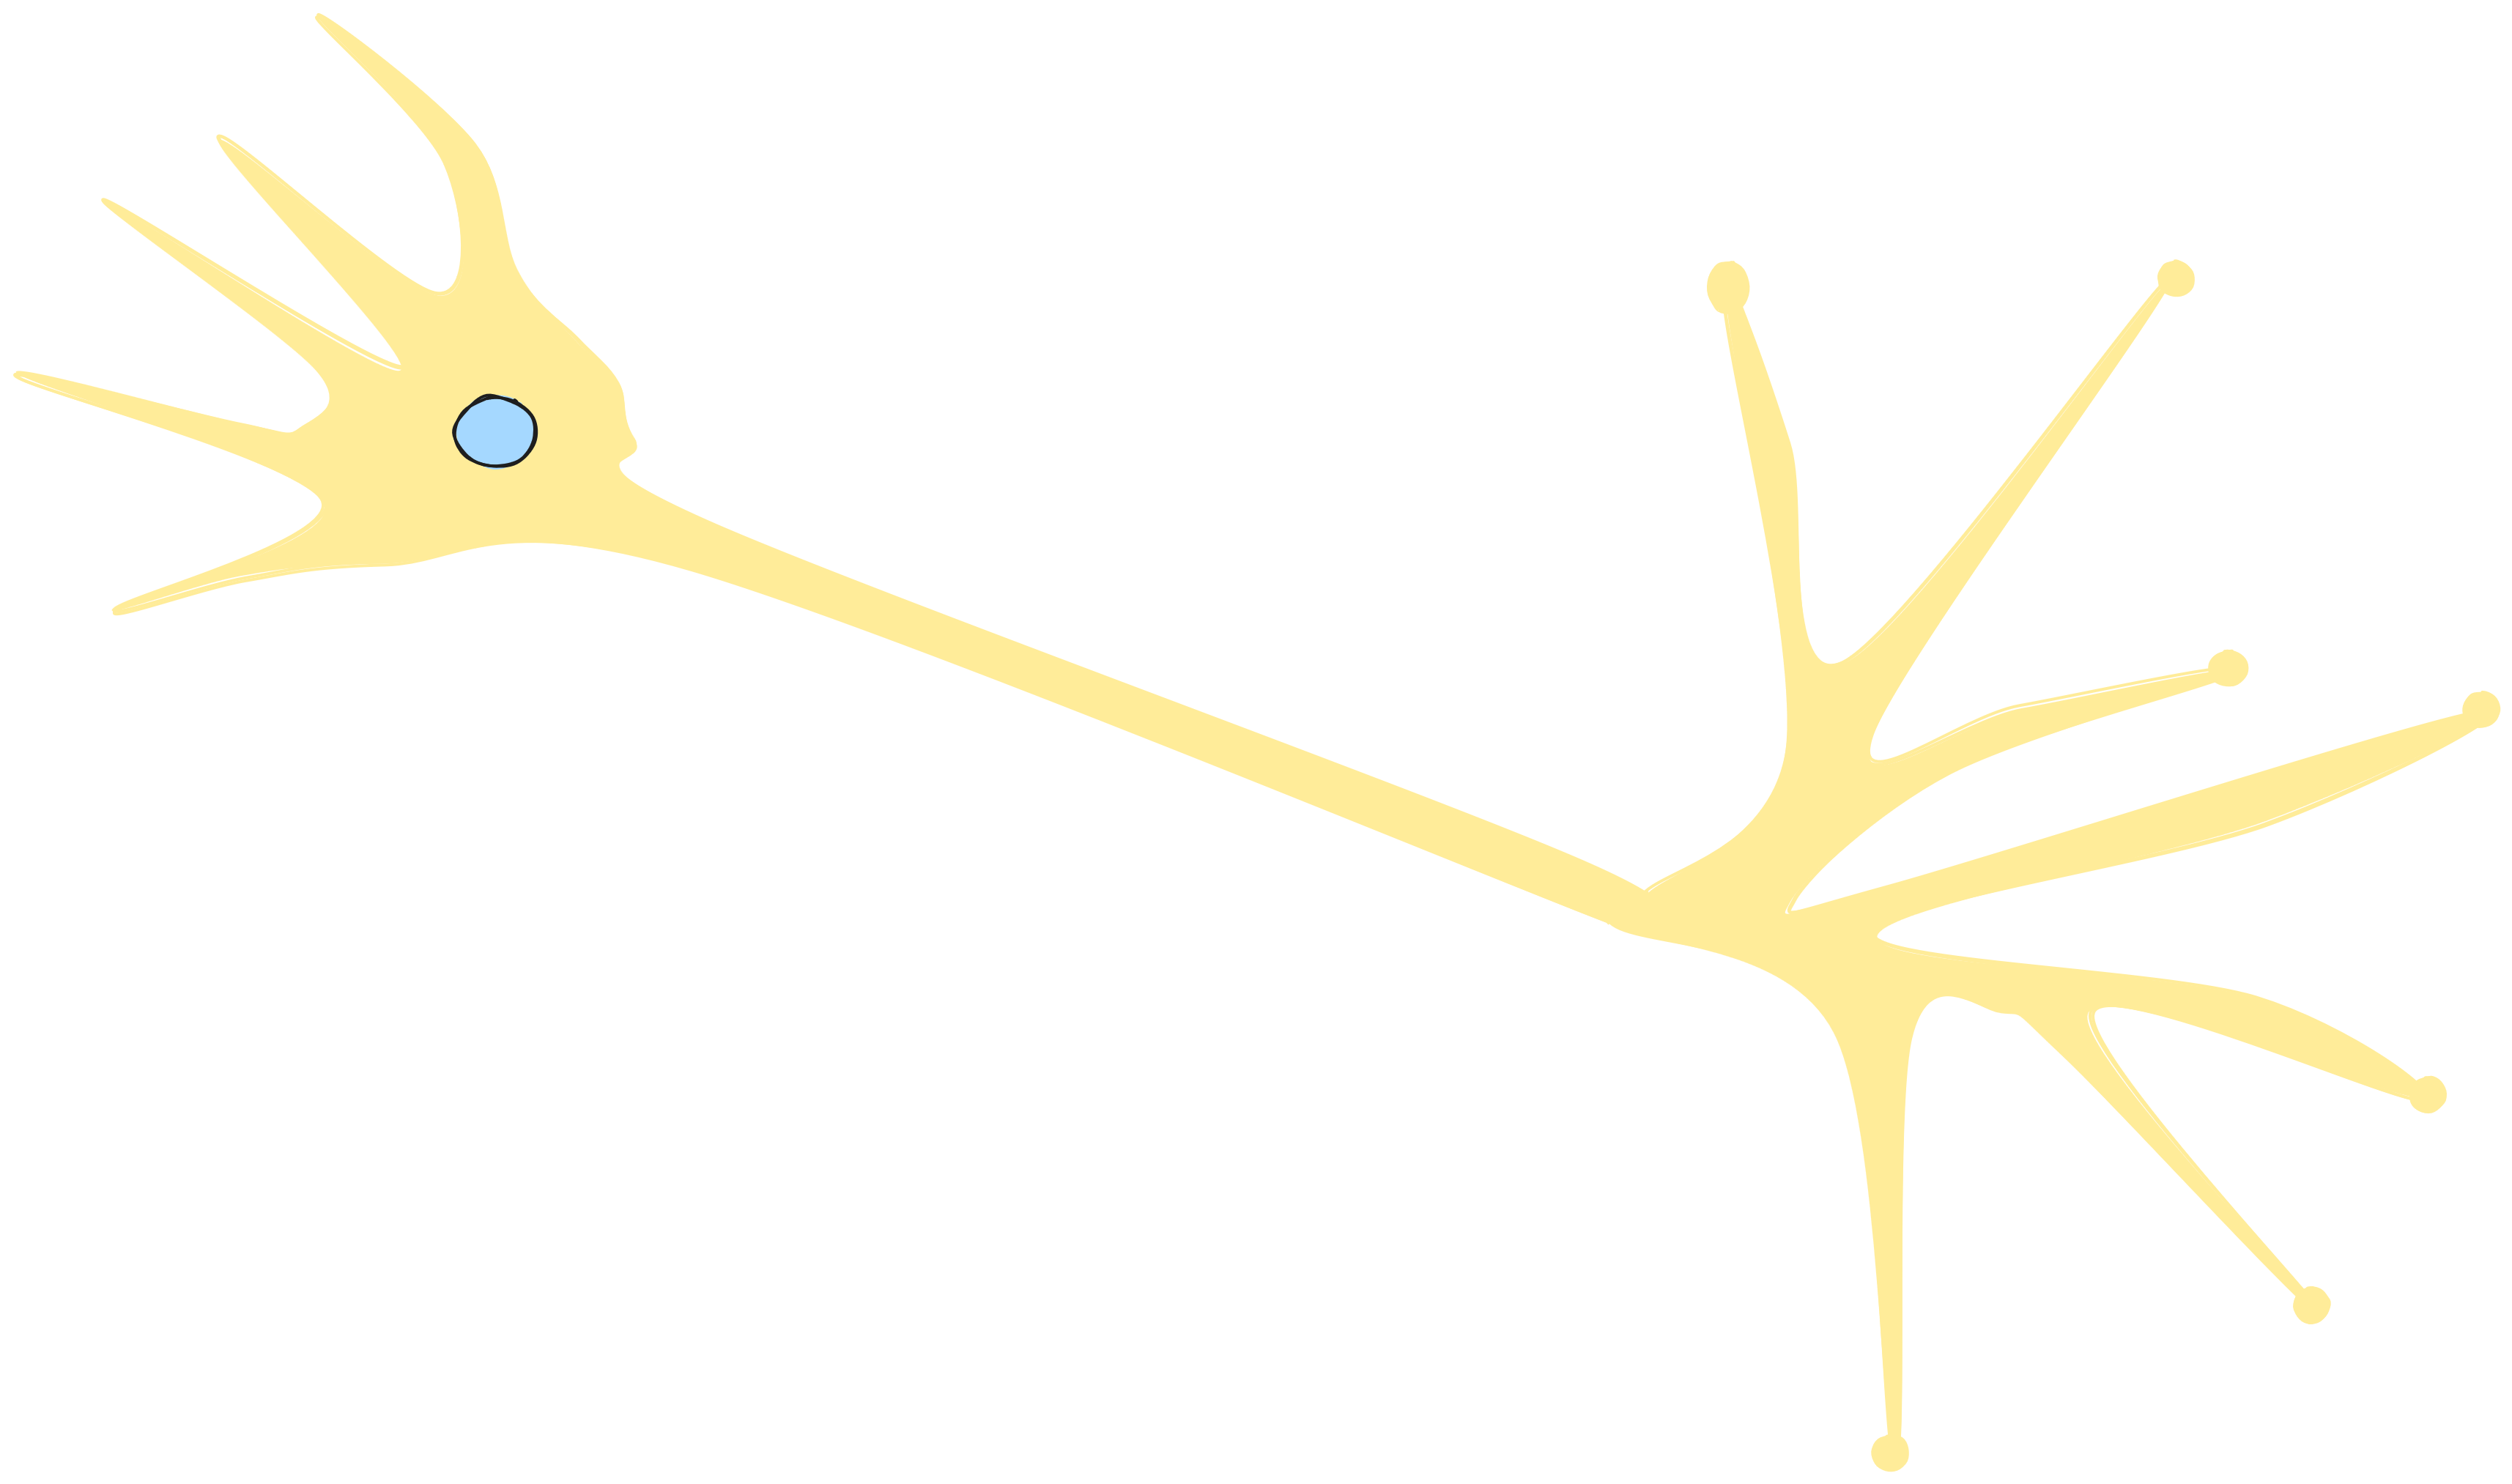
\includegraphics[width=0.5\textwidth]{nervcell.png}
\end{figure}

\begin{itemize}
    \item Beskriv de olika delarna av en nervcell och deras funktioner.
    \item Förklara hur en aktionspotential uppstår och fortplantas längs axonet.
\end{itemize}
\vspace{80mm}

\question \textbf{BONUS}: Beskriv något du lärt dig och tyckt varit extra intressant, men som inte var med på provet! (\textbf{2 bonuspoäng})

\end{questions}

\end{document}